\documentclass[UTF8]{ctexart}
\usepackage{mathtools,wallpaper}
\usepackage{lmodern}
\usepackage{t1enc}
\usepackage{pagecolor}
\usepackage{booktabs}
\usepackage{amsmath}
\usepackage{amsthm}
\usepackage{graphicx}
\renewcommand{\(}{\left(}
\renewcommand{\)}{\right)}
\begin{document}
\title{算法设计 HW01}  
\author{吴硕 522030910094}
\maketitle

\paragraph{Q1} 
In fact we can get that the reliability of the path from s to t is $\prod_{\(u,v\)\in{\(s,t\)}}^{}{p(u,v)}$
.As a result, we can use some tricks 
$$
\begin{aligned}
    \max\prod_{\(u,v\)\in{\(s,t\)}}^{}{p(u,v)}&=\max  {e^{\sum_{\(u,v\)\in{\(s,t\)}}^{}{\ln{p(u,v)}}}} \\
    &={e^{-\min\sum_{\(u,v\)\in{\(s,t\)}}^{}{-\ln{p(u,v)}}}} \\
\end{aligned}
$$
So, to get the most reliable path, we can just get the shortest path from s to t by making a new
graph $G^{1}$ with the weight of edge e(u,v) be $-\ln{p(u,v)}$.
Then we can use Dijkstra algorithm to get the shortest path from s to t in $G^{1}$.

The validity of this algorithm is obvious by Dijkstra algorithm.

The time complexity of this algorithm is $O\({\left| E\right|+\left| V\right|\log{\left| V\right|}}\)$ where E is the number of edges and V is the number of vertices by fibonacci heap..

\paragraph{Q2}

(a) We can make a graph by making a graph with just two vertices s and t and one edge between them. 

(b)  Because $G^{'}$ is strongly connected, we can get that there is a path from s to t and a path from t to s, and the two paths do not have the same edge.
If not, $G^{'}$ is not strongly connected. So, in graph G, any two vertices have two different paths between them, which have no common edges.
As a result, we can move any one edge from graph G and G is still connected.

(c) By the condition, we can know that in graph G, any two vertices have two different paths between them, which have no common edges.
Considering the graph $G^{'}$ and any vertices s and t in $G^{'}$. We can find the LCA of s and t, we can call
it v. Then because of the condition we can know that there are two paths between s and v, t and v in graph G. 
We call them a, b (between s and v), c, d (between t and v). WLOG, we assume that a and c are tree edges and b and
d are back edges. So we can get one path from s to t by b, c. And we can get another path from t to s by d, a. 
So, s and t are strongly connnected in $G^{'}$. Because of the arbitrariness of s and t, we can get that $G^{'}$ is strongly connected.

(d) Any graph G, we can just like the question that get $G^{'}$ by doing a DFS on G. 
Now considering $G^{'}$, if we delete the back edge, G is still connected by the tree edges. 
So, we can just selete the tree edge.

If we delete the tree edge e in path from s and t and there is a back edge from t to s. 
G is still connected. So, we can just delete the tree edge which is not in the range of any back edge. 
As a result, we can visit every back edge from t to s and add 1 to every tree edge from s to t. 
After that, all the tree edge of 0 is what we are looking for. 

The complexity: we first make a DFS on G, which is $O\({\left| E\right|+\left| V\right|}\)$. 
Then we can get the tree edge and back edge in $O\({\left| E\right|}\)$.
After that, we can get the result in $O\({\left| E\right|^{2}}\)$.
As a result, the total complexity is $O\({\left| V \right| + \left| E\right|^{2}}\)$.

\paragraph{Q3}

(a) The minimum number is $\max (\left| T(G) \right|, \left| H(G) \right|)$

If $\left|T(G)\right|>\left|H(G)\right|$ we assume H(G)={h1,h2,...,hm} and T(G)={t1,t2,...,tn}. 
So, we can add edges (t1,h1), (t2, h2)....(tm, hm), and (tm+1, h1),(tm+2, h1)...(tn, h1).
So any vertice s can reach a vertice ti in T(G) because DAG, so it can reach hi or h1. 
After that, it can reach any vertices in T(G). So, it can reach any vertices in H(G).
As a result, it can reach any vertices in G.

If $\left|T(G)\right|<=\left|H(G)\right|$ just similar to the above.

(b) Because G is not fullly reachable, so there exists h and t that t cannot be reached by h.
As a result, we can add (t,h). Because h can not reach t, so G is still a DAG.
What's more, by the edge, h is no loger a head and t is no loger a tail. So, the number of head and tail decrease by 1.

(c) By (a) and (b), we can easily solve this problem. 

First, we use (b) to and edges until it is fullly reachable. It is $O\(\left| E \right|\) $.

Then we use (a) to add edges until it is strongly connected.  It is $O\(\left| E \right|\) $.

The complexity is $O\({\left| E\right|}\)$.

(d) By tarjan algorithm ($O\({\left| V \right| + \left| E\right|}\)$), we can get the SCC of G. Then we can see every SCC as a vertice in a new graph G'.
Then we can get a new graph G' which is a DAG. Then we can use the above algorithm ($O\({\left| E\right|}\)$) to solve the problem.

So the complexity is $O\({\left| V \right| + \left| E\right|}\)$. 

\paragraph{Q4}

(a) If G is a good graph, consider it's DFS tree. Let e=(u,v) is a back edge. So, when u is visited in 
DFS, it choose another vertice. When u is visited in BFS, it must visit every vertice near u. So 
e must be added into BFS tree. So, G is not a good graph. This is a contradiction. So G has no back edge.
So G is a tree and it's DFS tree and BFS tree are both G. 

If G is a tree, it's DFS tree and BFS tree are both G. So G is a good graph.

(b) 
\begin{figure}[htbp]
    \centering
    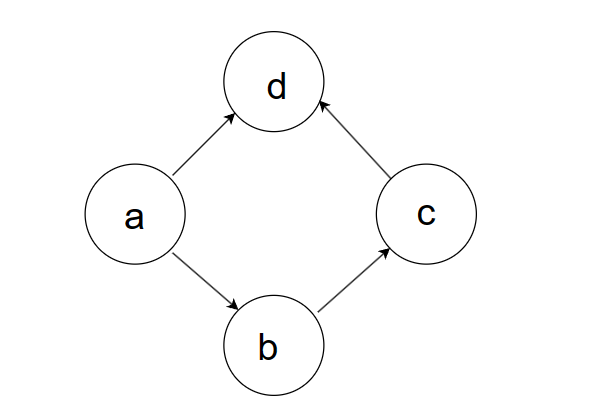
\includegraphics[width=6.5cm,height=5cm]{1.png}
    \end{figure} 

We can use this grapg to disaprove the statement.

a can reach every vertice in G.
And $\mathcal{L} =[a,b,d,c] or [a,d,b,c]$ by distacnce from a. 

$\mathcal{L} =[a,b,c,d]$ by topological order.

They are always different.

(c)
\begin{figure}[htbp]
    \centering
    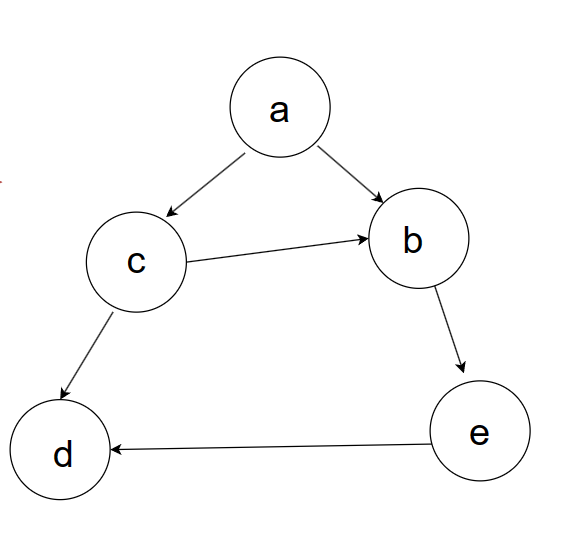
\includegraphics[width=6.5cm,height=5cm]{2.png}
    \end{figure} 

The topological order and length order are both [a,c,b,e,d]

However,the DFS and BFs tree are different.
Whenever we choose the order, BFS tree always has one kind :a->c->d,a->b->e;
But DFS tree can't be this shape.

\paragraph{Q5}
Consider making a BFS tree start from s.
Then, we give s's different subtres different colors. 
Then we can visit all notree edges.
If there is a notree edge (u,v) that u and v are in the same subtree, it count't form a cycle.
If there is a notree edge (u,v) that u and v are in different subtrees, it can form a cycle. And the size is $dep_u+dep_v+1$.
So we can just find the minimum size of the cycle.

complexity:BFS:$O(\left|E\right|+\left|V\right|)$

dye:$O(\left|E\right|)$

find the minimum size:$O(\left|E\right|)$

So the total complexity is $O(\left|E\right|+\left|V\right|)$

Correctness: All cycles must be consisted of al least one notree edge.

If there is a cycle consisted of more than one notree edge,because the BFS tree could find the shortest length
from s, so the cycle must larger than the minimum cycle.

So the minimum cycle must be consisted of only one notree edge and two tree edges.

What's more, by the above algorithm, we can find every cycle consisted of only one notree edge and two tree edges.

So we can find the minimum cycle.

(b) By a Dijkstra algorithm, we can get the shortest path from s to every vertice. 

So, just like above, we can form a shortest path tree and find the minimum cycle.

The correctness is similar to above.

The complexity is $O(\left|E\right|^{2})$ by Dijkstra.

\paragraph{Q6}

Time about 10 hours.

Difficulty: 5

Collaborator: 蒋松霖

\end{document}
